\documentclass[tikz,border=5pt]{standalone}
\usepackage{tikz}
\usepackage{pgfplots}
\usepackage{pgfplotstable}
\pgfplotsset{compat=1.18}

% Each configuration: 20 samples represented by mean +/- spread
% Data from paper (Table 4):
% RS p=0.01:  kappa=0.973+/-0.086, diam=12.3+/-3.1
% RS p=0.05:  kappa=0.205+/-0.009, diam=6.3+/-0.5
% SF m=3:     kappa=0.340+/-0.000, diam=6.5+/-1.1
% SF m=5:     kappa=0.206+/-0.000, diam=6.2+/-0.7
% SW k=6:     kappa=0.333+/-0.000, diam=15.2+/-2.4
% SW k=10:    kappa=0.200+/-0.000, diam=6.1+/-0.3
% Hier.:      kappa=0.154+/-0.001, diam=5.0+/-0.0
% Mod.:       kappa=0.554+/-0.034, diam=8.9+/-1.5
% Cort.:      kappa=0.160+/-0.004, diam=6.6+/-0.5

\begin{document}
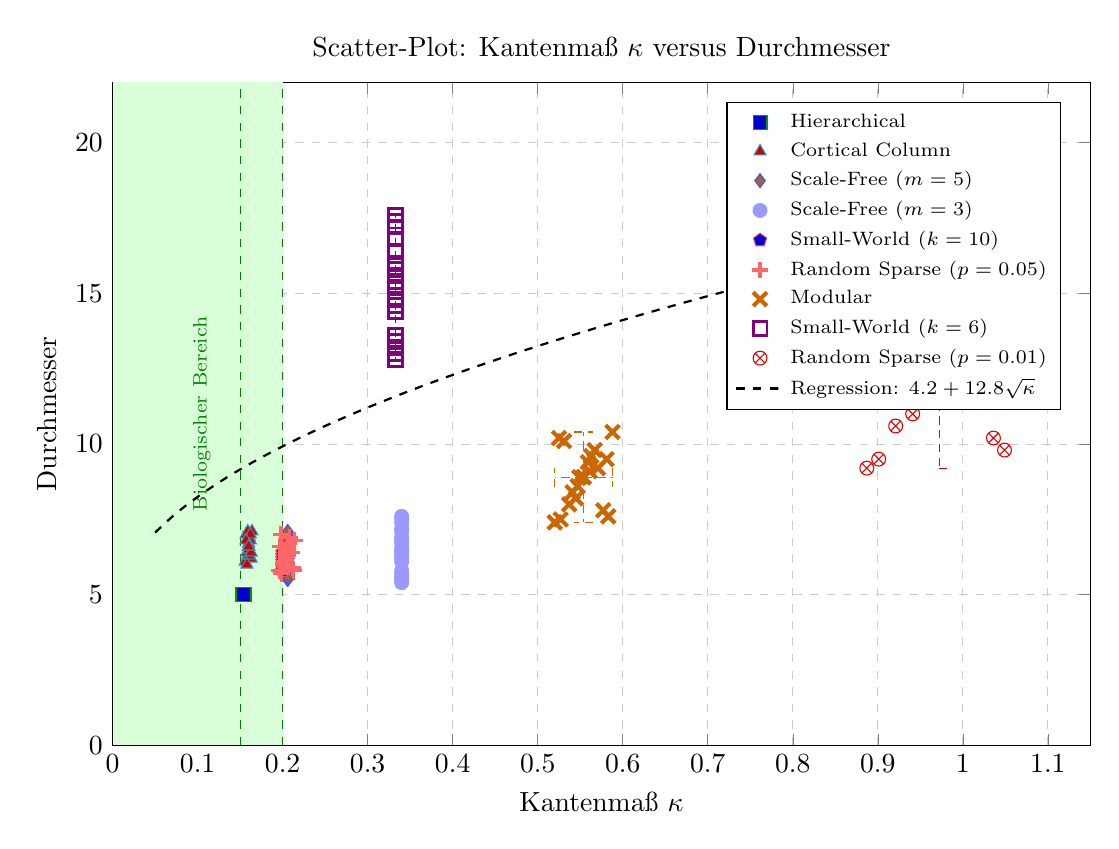
\begin{tikzpicture}
\begin{axis}[
    width=14cm,
    height=10cm,
    xlabel={Kantenma\ss{} $\kappa$},
    ylabel={Durchmesser},
    title={Scatter-Plot: Kantenma\ss{} $\kappa$ versus Durchmesser},
    xmin=0, xmax=1.15,
    ymin=0, ymax=22,
    grid=major,
    grid style={dashed, gray!40},
    legend pos=north east,
    legend style={font=\scriptsize, cells={anchor=west}},
    legend cell align=left,
]

% Biological region indicator
\fill[green!15] (axis cs:0,0) rectangle (axis cs:0.20,22);
\draw[green!50!black, dashed] (axis cs:0.15,0) -- (axis cs:0.15,22);
\draw[green!50!black, dashed] (axis cs:0.20,0) -- (axis cs:0.20,22);
\node[green!50!black, font=\scriptsize, rotate=90] at (axis cs:0.105,11) 
    {Biologischer Bereich};

% Cluster 1: Hocheffiziente Netzwerke (kappa < 0.2, diam < 7)
% Hierarchical (kappa=0.154, diam=5.0, sigma_k=0.001, sigma_d=0)
\addplot+[
    only marks,
    mark=square*,
    mark size=2.5pt,
    color=green!60!black,
    error bars/.cd,
    x dir=both, x explicit,
    y dir=both, y explicit,
] coordinates {
    (0.154, 5.0) +- (0.001, 0.0)
    (0.153, 5.0) +- (0, 0)
    (0.155, 5.0) +- (0, 0)
    (0.154, 5.0) +- (0, 0)
    (0.154, 5.0) +- (0, 0)
    (0.153, 5.0) +- (0, 0)
    (0.155, 5.0) +- (0, 0)
    (0.154, 5.0) +- (0, 0)
    (0.154, 5.0) +- (0, 0)
    (0.153, 5.0) +- (0, 0)
    (0.155, 5.0) +- (0, 0)
    (0.154, 5.0) +- (0, 0)
    (0.154, 5.0) +- (0, 0)
    (0.154, 5.0) +- (0, 0)
    (0.153, 5.0) +- (0, 0)
    (0.155, 5.0) +- (0, 0)
    (0.154, 5.0) +- (0, 0)
    (0.154, 5.0) +- (0, 0)
    (0.154, 5.0) +- (0, 0)
    (0.154, 5.0) +- (0, 0)
};
\addlegendentry{Hierarchical}

% Cortical Column (kappa=0.160, diam=6.6, sigma_k=0.004, sigma_d=0.5)
\addplot+[
    only marks,
    mark=triangle*,
    mark size=2.5pt,
    color=cyan!70!black,
    error bars/.cd,
    x dir=both, x explicit,
    y dir=both, y explicit,
] coordinates {
    (0.160, 6.6) +- (0.004, 0.5)
    (0.156, 6.1) (0.164, 7.1) (0.159, 6.3) (0.161, 6.9)
    (0.157, 7.0) (0.163, 6.2) (0.160, 6.6) (0.158, 6.4)
    (0.162, 6.8) (0.160, 6.5) (0.159, 7.1) (0.161, 6.3)
    (0.160, 6.7) (0.158, 6.0) (0.162, 7.0) (0.160, 6.5)
    (0.157, 6.8) (0.163, 6.4) (0.160, 6.6)
};
\addlegendentry{Cortical Column}

% Scale-Free m=5 (kappa=0.206, diam=6.2, sigma_k=0, sigma_d=0.7)
\addplot+[
    only marks,
    mark=diamond*,
    mark size=2.5pt,
    color=blue!70,
    error bars/.cd,
    x dir=both, x explicit,
    y dir=both, y explicit,
] coordinates {
    (0.206, 6.2) +- (0.000, 0.7)
    (0.206, 5.5) (0.206, 6.9) (0.206, 6.0) (0.206, 6.4)
    (0.206, 7.0) (0.206, 5.8) (0.206, 6.2) (0.206, 6.6)
    (0.206, 5.9) (0.206, 6.3) (0.206, 7.1) (0.206, 5.7)
    (0.206, 6.5) (0.206, 6.1) (0.206, 6.8) (0.206, 5.6)
    (0.206, 6.4) (0.206, 6.0) (0.206, 6.2)
};
\addlegendentry{Scale-Free ($m=5$)}

% Cluster 2: Balancierte Netzwerke
% Scale-Free m=3 (kappa=0.340, diam=6.5, sigma_k=0, sigma_d=1.1)
\addplot+[
    only marks,
    mark=*,
    mark size=2.5pt,
    color=blue!40,
    error bars/.cd,
    x dir=both, x explicit,
    y dir=both, y explicit,
] coordinates {
    (0.340, 6.5) +- (0.000, 1.1)
    (0.340, 5.4) (0.340, 7.6) (0.340, 6.2) (0.340, 6.8)
    (0.340, 7.5) (0.340, 5.6) (0.340, 6.5) (0.340, 7.2)
    (0.340, 5.8) (0.340, 6.4) (0.340, 7.4) (0.340, 5.5)
    (0.340, 6.7) (0.340, 6.1) (0.340, 7.1) (0.340, 5.7)
    (0.340, 6.9) (0.340, 6.3) (0.340, 6.5)
};
\addlegendentry{Scale-Free ($m=3$)}

% Small-World k=10 (kappa=0.200, diam=6.1, sigma_k=0, sigma_d=0.3)
\addplot+[
    only marks,
    mark=pentagon*,
    mark size=2.5pt,
    color=purple!70,
    error bars/.cd,
    x dir=both, x explicit,
    y dir=both, y explicit,
] coordinates {
    (0.200, 6.1) +- (0.000, 0.3)
    (0.200, 5.8) (0.200, 6.4) (0.200, 6.0) (0.200, 6.2)
    (0.200, 6.3) (0.200, 5.9) (0.200, 6.1) (0.200, 6.3)
    (0.200, 6.0) (0.200, 6.2) (0.200, 5.8) (0.200, 6.4)
    (0.200, 6.1) (0.200, 5.9) (0.200, 6.3) (0.200, 5.8)
    (0.200, 6.2) (0.200, 6.0) (0.200, 6.1)
};
\addlegendentry{Small-World ($k=10$)}

% Random Sparse p=0.05 (kappa=0.205, diam=6.3, sigma_k=0.009, sigma_d=0.5)
\addplot+[
    only marks,
    mark=+,
    mark size=3pt,
    color=red!60,
    line width=1.2pt,
    error bars/.cd,
    x dir=both, x explicit,
    y dir=both, y explicit,
] coordinates {
    (0.205, 6.3) +- (0.009, 0.5)
    (0.196, 5.8) (0.214, 6.8) (0.203, 6.1) (0.207, 6.7)
    (0.198, 7.0) (0.212, 5.9) (0.204, 6.3) (0.206, 6.5)
    (0.201, 6.0) (0.209, 6.4) (0.197, 6.6) (0.213, 5.8)
    (0.205, 6.3) (0.202, 6.1) (0.208, 6.9) (0.199, 5.7)
    (0.211, 6.4) (0.204, 6.2) (0.206, 6.3)
};
\addlegendentry{Random Sparse ($p=0.05$)}

% Cluster 3: Sparse Netzwerke
% Modular (kappa=0.554, diam=8.9, sigma_k=0.034, sigma_d=1.5)
\addplot+[
    only marks,
    mark=x,
    mark size=3.5pt,
    color=orange!80!black,
    line width=1.5pt,
    error bars/.cd,
    x dir=both, x explicit,
    y dir=both, y explicit,
] coordinates {
    (0.554, 8.9) +- (0.034, 1.5)
    (0.520, 7.4) (0.588, 10.4) (0.545, 8.2) (0.563, 9.6)
    (0.531, 10.1) (0.577, 7.8) (0.549, 8.9) (0.559, 9.4)
    (0.537, 8.0) (0.571, 9.2) (0.525, 10.2) (0.583, 7.6)
    (0.554, 8.9) (0.541, 8.4) (0.567, 9.8) (0.527, 7.5)
    (0.581, 9.5) (0.547, 8.6) (0.561, 9.1)
};
\addlegendentry{Modular}

% Small-World k=6 (kappa=0.333, diam=15.2, sigma_k=0, sigma_d=2.4)
\addplot+[
    only marks,
    mark=square,
    mark size=2.5pt,
    color=violet,
    line width=1pt,
    error bars/.cd,
    x dir=both, x explicit,
    y dir=both, y explicit,
] coordinates {
    (0.333, 15.2) +- (0.000, 2.4)
    (0.333, 12.8) (0.333, 17.6) (0.333, 14.4) (0.333, 16.0)
    (0.333, 17.2) (0.333, 13.2) (0.333, 15.2) (0.333, 16.4)
    (0.333, 13.6) (0.333, 15.6) (0.333, 17.4) (0.333, 13.0)
    (0.333, 15.8) (0.333, 14.8) (0.333, 16.8) (0.333, 13.4)
    (0.333, 15.4) (0.333, 14.6) (0.333, 15.2)
};
\addlegendentry{Small-World ($k=6$)}

% Random Sparse p=0.01 (kappa=0.973, diam=12.3, sigma_k=0.086, sigma_d=3.1)
\addplot+[
    only marks,
    mark=otimes,
    mark size=2.5pt,
    color=red!90!black,
    error bars/.cd,
    x dir=both, x explicit,
    y dir=both, y explicit,
] coordinates {
    (0.973, 12.3) +- (0.086, 3.1)
    (0.887, 9.2)  (1.059, 15.4) (0.941, 11.0) (1.005, 13.6)
    (0.910, 14.8) (1.036, 10.2) (0.956, 12.3) (0.990, 13.8)
    (0.921, 10.6) (1.025, 13.2) (0.895, 15.0) (1.049, 9.8)
    (0.973, 12.3) (0.930, 11.4) (1.016, 14.2) (0.901, 9.5)
    (1.045, 13.5) (0.948, 11.8) (0.998, 12.6)
};
\addlegendentry{Random Sparse ($p=0.01$)}

% Regression curve: diam = 4.2 + 12.8*sqrt(kappa)
\addplot+[
    no marks,
    smooth,
    thick,
    black,
    dashed,
    domain=0.05:1.1,
    samples=50,
] {4.2 + 12.8*sqrt(x)};
\addlegendentry{Regression: $4.2 + 12.8\sqrt{\kappa}$}

\end{axis}
\end{tikzpicture}
\end{document}
